\documentclass[12pt, a4paper, oneside]{book}
\usepackage[hidelinks]{hyperref}
\usepackage[slovak]{babel}
\usepackage{epsfig}
\usepackage{epstopdf}
\usepackage[chapter]{algorithm}
\usepackage{algorithmic}
\usepackage{listings}
\usepackage{amsmath}
\usepackage{amssymb}
\usepackage{graphicx}
\usepackage{multirow}
\usepackage{color}
\usepackage{url}
\usepackage[utf8]{inputenc}
\usepackage[T1]{fontenc}
\usepackage{setspace}
\usepackage{tabularx}
\usepackage{textcomp}
\usepackage{caption}
\usepackage{natbib}

\setstretch{1.5}
%\renewcommand\baselinestretch{1.5} % riadkovanie jeden a pol

% pekne pokope definujeme potrebne udaje
\newcommand\mftitle{Model na simuláciu peny}
\newcommand\mfthesistype{Diplomová práca}
\newcommand\mfauthor{Bc. Viktor Nagy}
\newcommand\mfadvisor{prof. RNDr. Jiri Silha, PhD.}
\newcommand\mfplacedate{Bratislava, 2014}
\newcommand\mfuniversity{UNIVERZITA KOMENSKÉHO V BRATISLAVE}
\newcommand\mffaculty{FAKULTA MATEMATIKY, FYZIKY A INFORMATIKY}
\newcommand{\sub}[1]{$_{\text{#1}}$}
\newcommand{\reference}[1]{č.~\ref{#1}}
\newcommand{\imageHeight}{150px}

\ifx\pdfoutput\undefined\relax\else\pdfinfo{ /Title (\mftitle) /Author (\mfauthor) /Creator (PDFLaTeX) } \fi

\begin{document}

\frontmatter

\thispagestyle{empty}

\noindent
\begin{minipage}{\textwidth}
\begin{center}
\textbf{\mfuniversity \\
\mffaculty}
\end{center}
\end{minipage}

\vfill
\begin{figure}[!hbt]
	\begin{center}
		
\includegraphics{images/logo_fmph}
		\label{img:logo}
	\end{center}
\end{figure}
\begin{center}
	\begin{minipage}{0.8\textwidth}
		\centerline{\textbf{\Large\MakeUppercase{\mftitle}}}
		\smallskip
		\centerline{\mfthesistype}
	\end{minipage}
\end{center}
\vfill
2014 \hfill
\mfauthor
\eject 
% koniec obalu

\thispagestyle{empty}

\noindent
\begin{minipage}{\textwidth}
\begin{center}
\textbf{\mfuniversity \\
\mffaculty}
\end{center}
\end{minipage}

\vfill
\begin{figure}[!hbt]
\begin{center}

\includegraphics{images/logo_fmph_dark}
\label{img:logo_dark}
\end{center}
\end{figure}
\begin{center}
\begin{minipage}{0.8\textwidth}
\centerline{\textbf{\Large\MakeUppercase{\mftitle}}}
\smallskip
\centerline{\mfthesistype}
\end{minipage}
\end{center}
\vfill
\begin{tabular}{l l}
%Registration number: & 40a99bd8-3cb6-4534-9330-c7fd9b5e5ca4 \\
Študijný program: & Aplikovaná informatika\\
Študijný odbor: & 2511 Aplikovaná informatika\\
Školiace pracovisko: & Katedra aplikovanej informatiky\\
Školiteľ: & \mfadvisor
\end{tabular}
\vfill
\noindent
\mfplacedate \hfill
\mfauthor
\eject 
% koniec titulneho listu

%\thispagestyle{empty}
%\includegraphics[width=\textwidth]{images/zadanie}
%\vfill
%\eject
% koniec zadania

\thispagestyle{empty}


\begin{figure}[H]
\begin{center}
\makebox[\textwidth]{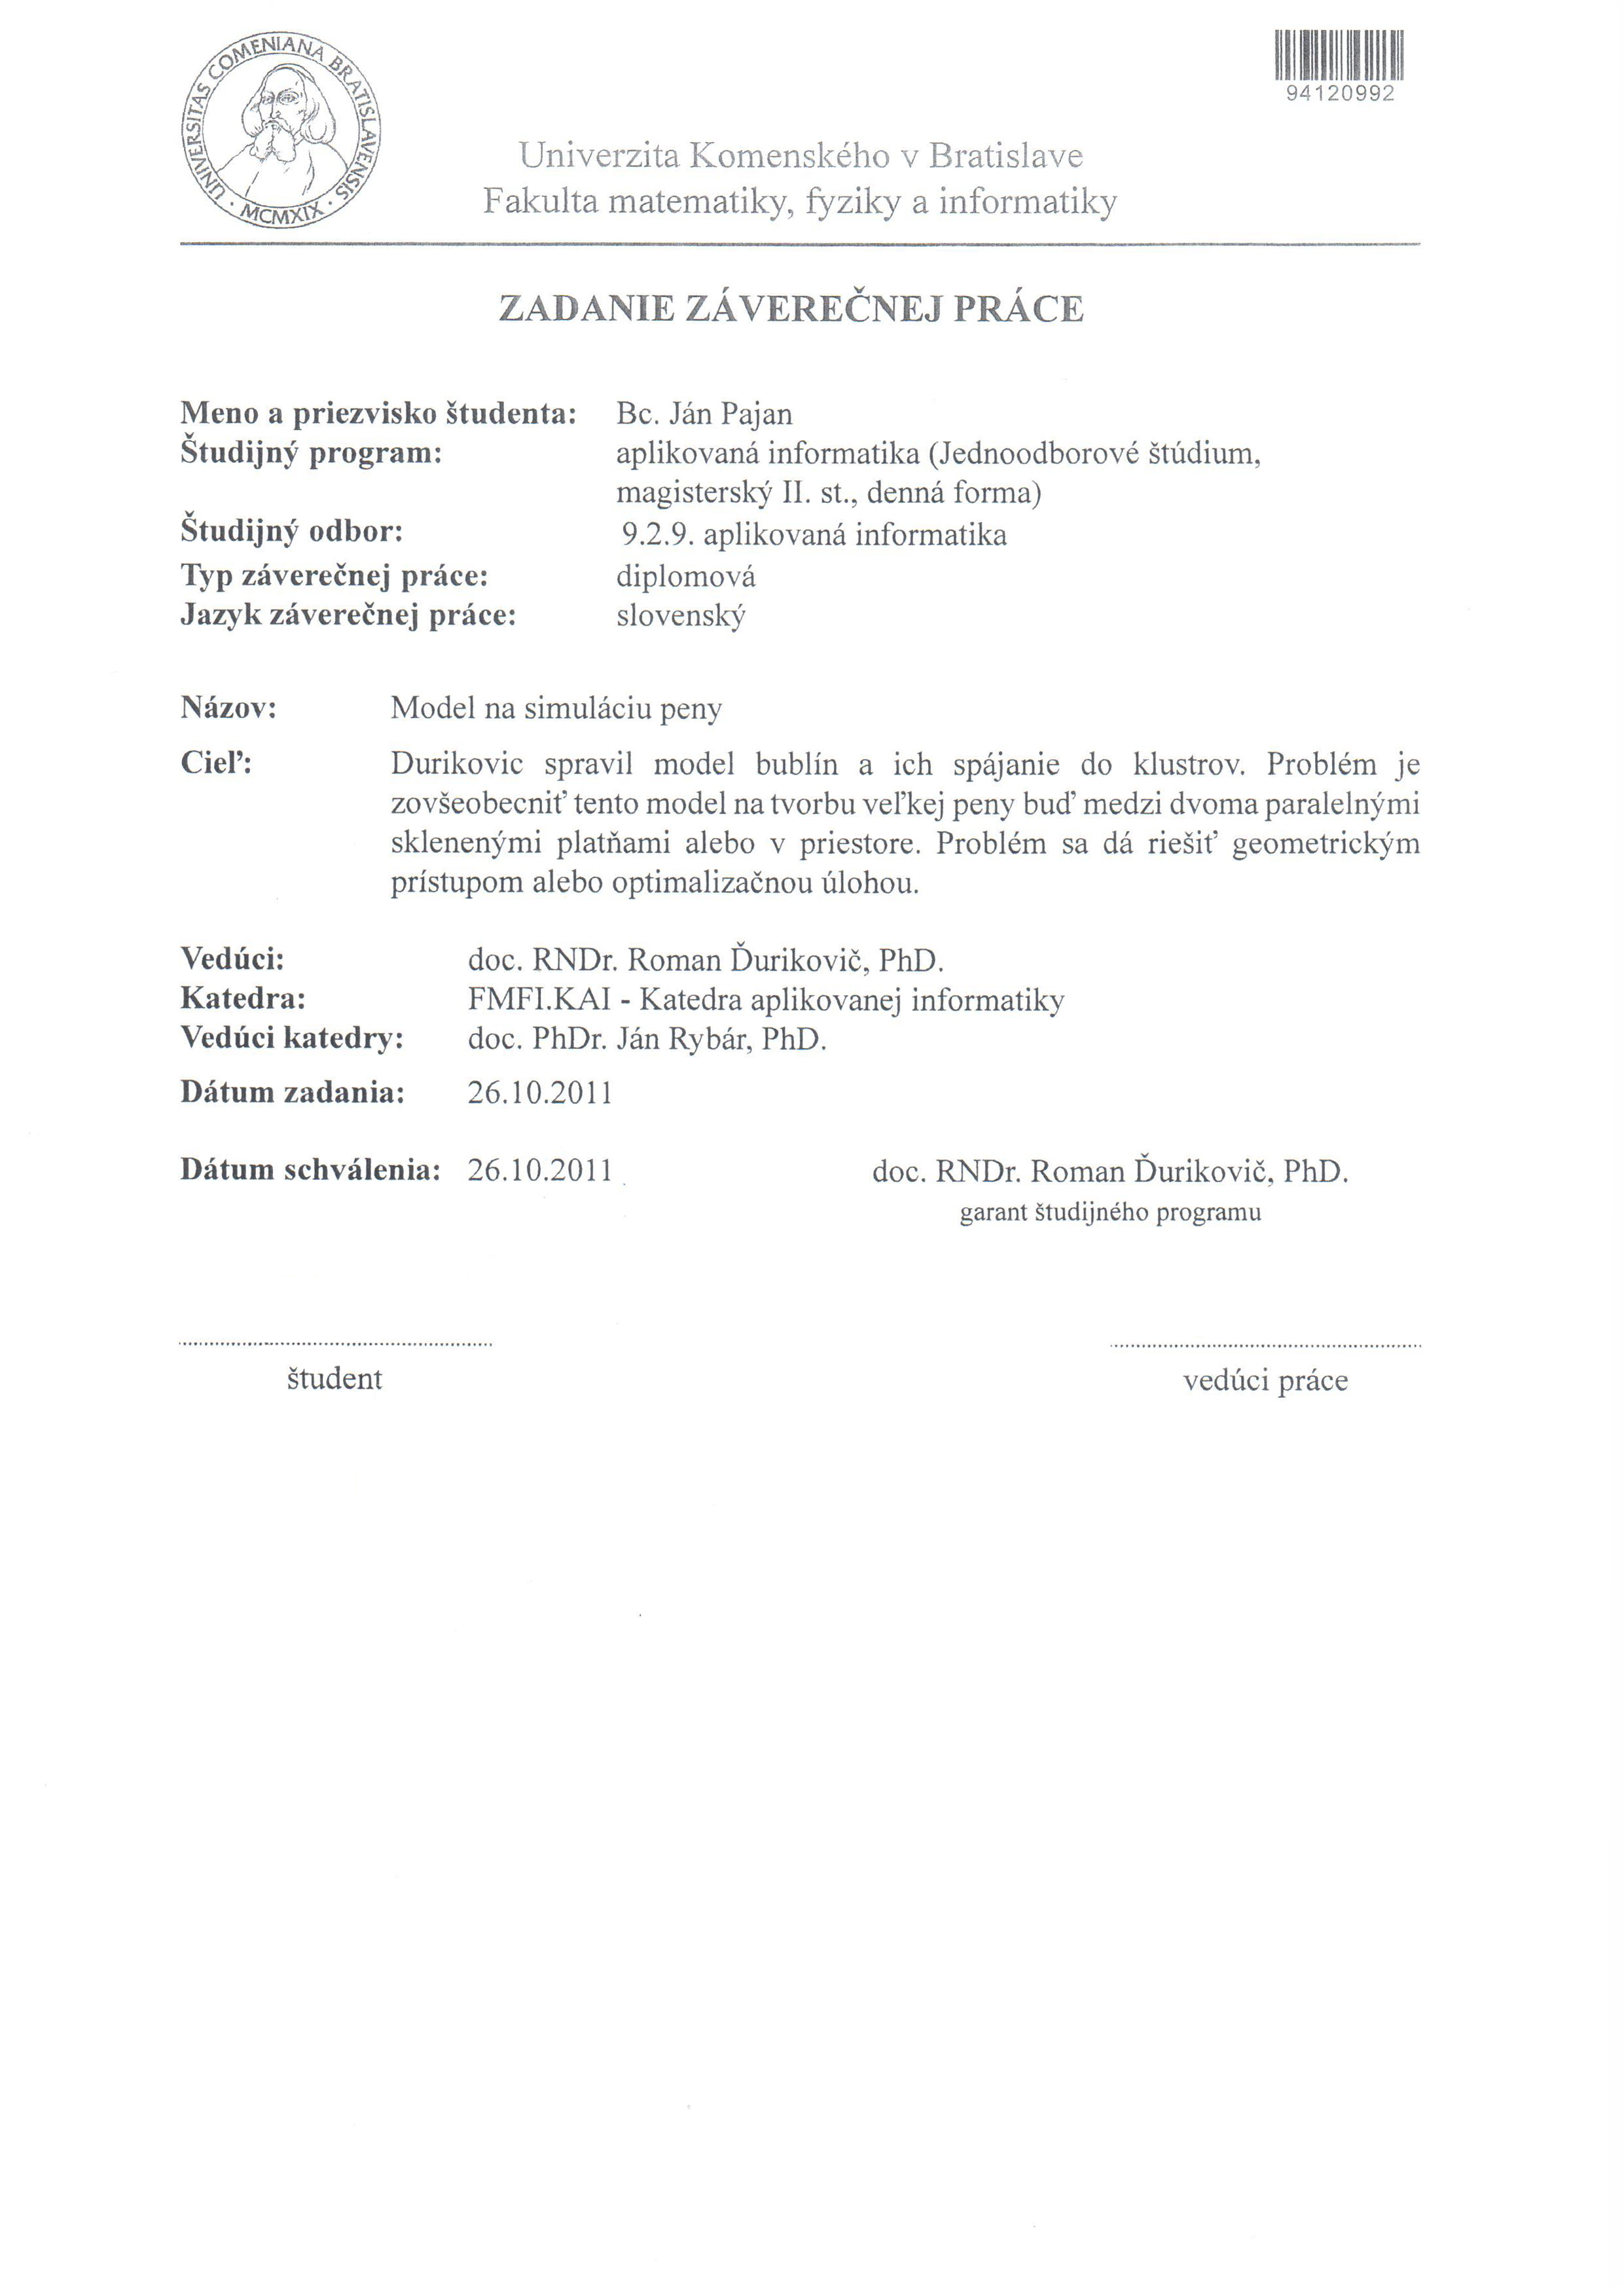
\includegraphics[width=\paperwidth]{images/zadaniedp}}
\label{img:zadanie}
\end{center}
\end{figure}

{~}\vspace{12cm}

\noindent
\begin{minipage}{0.25\textwidth}~\end{minipage}
\begin{minipage}{0.75\textwidth}
Čestne prehlasujem, že túto diplomovú prácu som vypracoval samostatne len s použitím uvedenej literatúry a za pomoci konzultácií u môjho školiteľa.
\newline \newline
\end{minipage}
\vfill
~ \hfill {\hbox to 6cm{\dotfill}} \\
\mfplacedate \hfill \mfauthor
\vfill\eject 
% koniec prehlasenia

\chapter*{Poďakovanie}\label{chap:thank_you}
Touto cestou by som sa chcel v prvom rade poďakovať môjmu školiteľovi prof. RNDr. Romanovi Ďurikovičovi, PhD. za jeho cenné rady a usmernenia, ktoré mi veľmi pomohli pri riešení tejto diplomovej práce. Takisto sa chcem poďakovať mojím kolegom z YACGS semináru za rady ohľadom implementácie a v neposlednom rade chcem tiež poďakovať všetkým mojím kamarátom a celej mojej rodine za podporu počas môjho štúdia. 
\vfill\eject 
% koniec podakovania

\chapter*{Abstrakt}\label{chap:abstract_sk}
Táto práca sa venuje problematike simulácie peny a bublín, z ktorých táto pena pozostáva. Súčasťou tejto práce je prehľad existujúcich riešení a ich krátke zhodnotenie. Ďalej je tu popísaný návrh a implementácia nášho modelu inšpirovaného niektorými zaujímavými riešeniami z dvoch existujúcich modelov, ktorý je založený na princípe pružinového systému. Simulácia je riešená implicitnou metódu s využitím spätnej Eulerovej metódy, ktorá počíta rýchlosti bublín v ďalšom časovom kroku. Na deformáciu dotýkajúcich sa bublín je využitý vertex shader a realistické zobrazenie bublín umocňuje použitie techniky zvanej "cube mapping" kombinovanej s alpha blendingom. Prínosom nášho riešenia je najmä vytváranie animácii simulujúcich tzv. "Bubble Show".

~\\
Kľúčové slová: simulácia peny, vizualizácia peny
\vfill\eject 

\chapter*{Abstract}\label{chap:abstract_en}
This thesis deals with foam simulation issues. This work also contains an overview of existing solutions and short summary to each of them. In the next part we describe proposal and implementation of our model, which is inspired by some interesting solutions from two existing models. Our model is based on spring system principle. Simulation uses implicit method which uses backward Euler method to compute bubble velocities at the next time step. Deformation of touching bubbles is handled by vertex shader and the realistic visualization of bubbles is achieved by using technique called "cubbe mapping", which is combined with alpha blending. Asset of our solution is mainly in generation of animations that simulate "Bubble Show".

~\\
Keywords: foam simulation, foam rendering
\vfill\eject 
% koniec abstraktov

\tableofcontents

\mainmatter

% treba este prejst dokument ci je kod spravne formatovany
\input 01intro.tex
\input 02motivation.tex
\input 03issues_overview.tex
\input 04previous_solutions.tex
\input 05proposal.tex
\input 06implementation.tex
\input 07results.tex
\input 08conclusion.tex

\backmatter

\nocite{*}
\bibliographystyle{alpha}
\bibliography{references}

\listoffigures

\end{document}
